\subsection{Integration Strategy with RTC Systems}

The integration strategy defines how the proposed audio deepfake detection service is connected to real-world real-time communication (RTC) environments without requiring modifications to the core RTC application. Since many RTC platforms, including WebRTC-based systems, VoIP services, and conferencing applications, operate as closed or partially restricted ecosystems, the proposed detector is designed as an external service-oriented component that interfaces with the RTC pipeline through standardized audio streaming access points.

\vspace{0.5cm}
\begin{figure}[H]
    \centering
    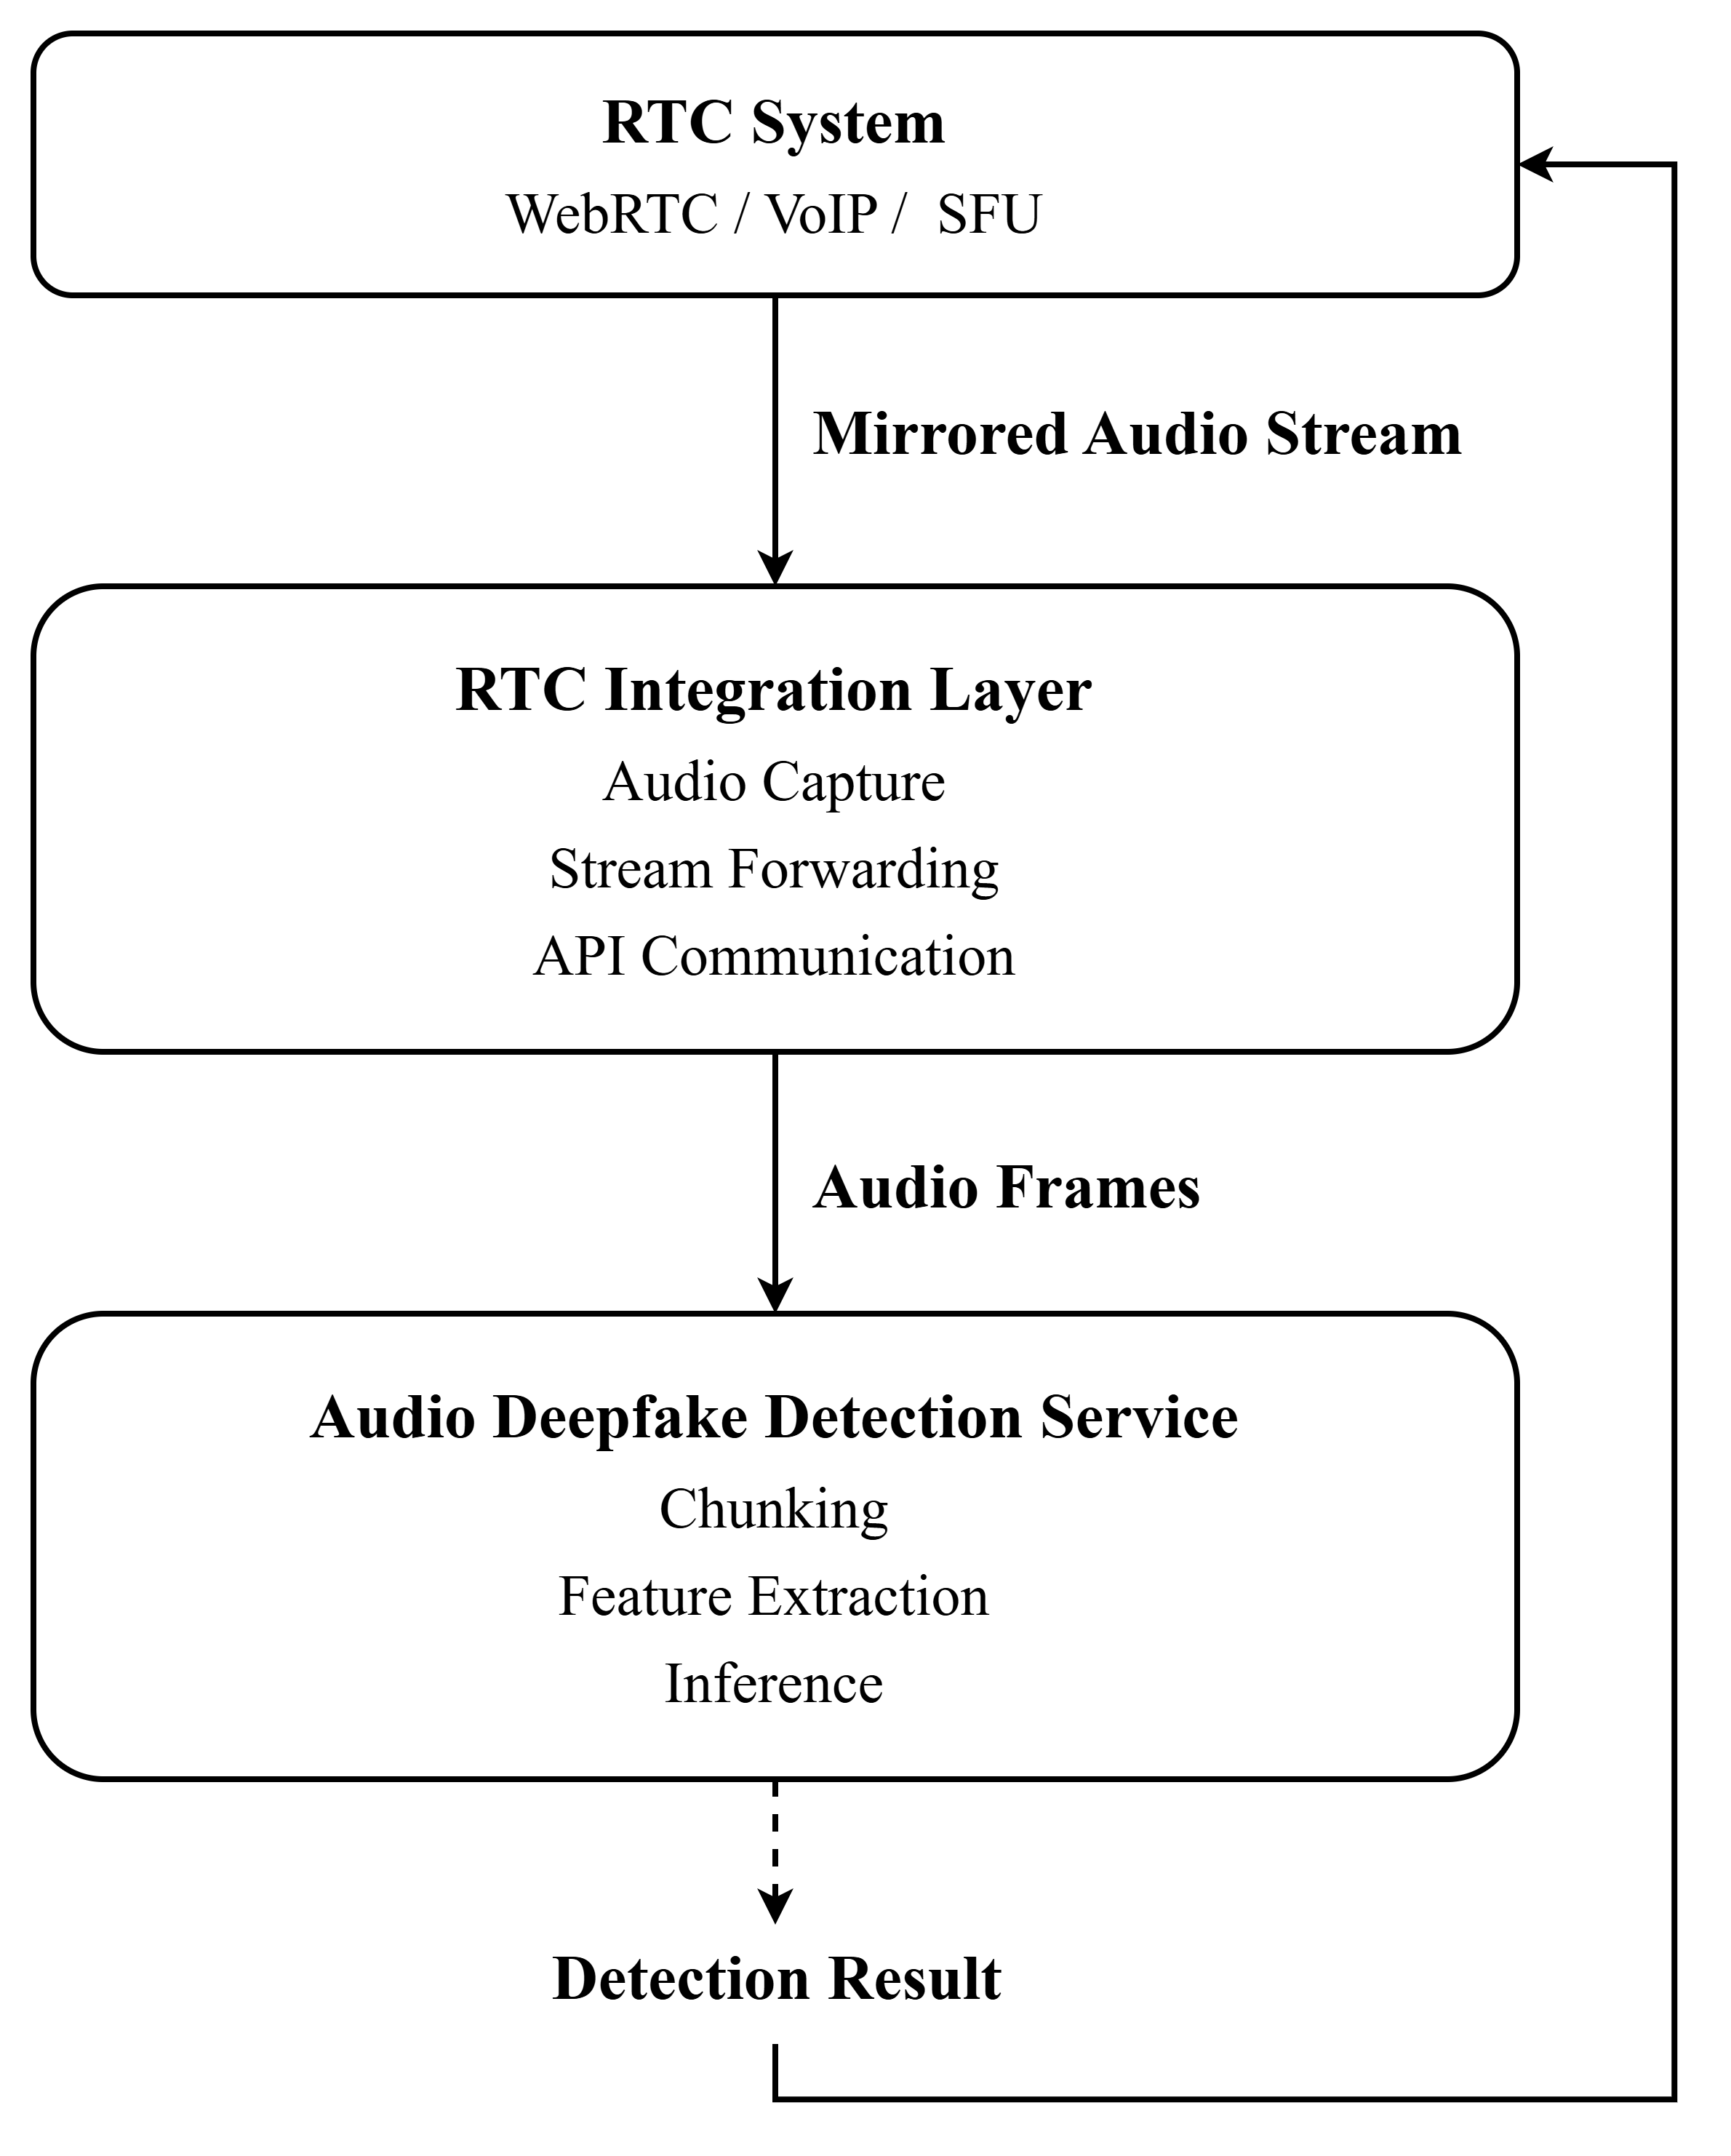
\includegraphics[width=0.7\textwidth]{images/methodology/integration_strategy.png}
    \vspace{0.25cm}
    \caption{Integration of Detection Service with RTC systems}
    \label{fig:integration_strategy}
\end{figure}

The primary objective of this integration layer is to enable continuous detection on reconstructed audio streams while preserving the real-time properties of the communication system. The detector is therefore deployed as a parallel inference component rather than as an in-band modification of the RTC stack.

\subsubsection{Deployment Modes}

Two deployment configurations are considered for integrating the detection service into RTC environments.

In the \textbf{client-side deployment}, a lightweight agent or SDK is embedded within the developed RTC application environment. This agent captures reconstructed audio on the receiver side and forwards audio chunks to the detection service for inference. This approach can provide fast response times and low network overhead; however, it is limited by device compute capacity, deployment complexity, and privacy constraints.

In the \textbf{server-side deployment}, which is the preferred configuration in this work, audio is intercepted at the media server or selective forwarding unit (SFU) level after decoding and jitter-buffer processing. The detection service then consumes mirrored audio streams centrally, enabling consistent processing across multiple sessions while avoiding the computational burden on end-user devices. This approach is particularly suitable for enterprise RTC systems and server-managed communication platforms.

\subsubsection{Integration Point in the RTC Pipeline}

The proposed detector is attached at the stage where audio has already been reconstructed into a stable waveform representation. This point is typically located after receiver-side decoding and enhancement, or at the output of a media server that forwards a mirrored copy of the stream.

The detector operates as a passive observer of the reconstructed audio stream and does not alter the primary communication path. This design ensures that deepfake analysis does not degrade call quality or introduce interference in the RTC session.

Technically, the integration may be realized using RTP stream duplication, media server hooks, audio tap points, or WebRTC-compatible plugin mechanisms, depending on the target deployment environment.

\subsubsection{API-Based Communication Workflow}

Communication between the developed RTC system and the detection service is handled through a streaming API layer, typically implemented using gRPC for low-latency environments or HTTP-based streaming for simpler deployments.

The workflow follows a chunk-based streaming model in which reconstructed audio segments are transmitted to the detection service in near real time. Each chunk is processed independently, while a small temporal buffer is maintained to preserve continuity across adjacent windows.

Let the reconstructed audio stream be represented as \(x_{out}[n]\). The integration layer segments this stream into chunks
\begin{equation}
X = \{x_1, x_2, \ldots, x_T\},
\end{equation}
which are transmitted to the detector through the API channel.

For each input chunk, the service returns an inference result consisting of a spoofing probability and an associated class label. This request-response design keeps the detector platform-agnostic and avoids dependency on specific codec or transport implementations.

\subsubsection{Scalability and Latency Considerations}

RTC applications impose strict latency requirements, so the detection system is designed to operate under bounded inference delay. To maintain responsiveness, the service processes fixed-size audio chunks instead of full utterances and uses compact feature extractors at runtime.

Scalability is achieved through horizontal replication of the detection service behind a load balancer. This allows multiple concurrent RTC sessions to be processed in parallel without significant performance degradation. To further reduce runtime overhead, heavy feature extraction components may rely on pretrained encoders that remain frozen during inference. This design balances detection accuracy with real-time constraints and ensures that the system can operate reliably in live RTC environments.